\documentclass[aspectratio=169]{beamer}
%
% Choose how your presentation looks.
%
% For more themes, color themes and font themes, see:
% http://deic.uab.es/~iblanes/beamer_gallery/index_by_theme.html
%
\mode<presentation>
{
  \usetheme{metropolis}      % or try Darmstadt, Madrid, Warsaw, ...
  \usecolortheme{metropolis-imagelab} % or try albatross, beaver, crane, ...
  \usefonttheme{structurebold}  % or try serif, structurebold, ...
  \setbeamercolor{background canvas}{bg=white}
  \setbeamertemplate{navigation symbols}{}
  \setbeamertemplate{bibliography item}{\insertbiblabel}
  %\setbeamertemplate{caption}[numbered]
} 
\usepackage[english]{babel}
\usepackage[utf8x]{inputenc}
\usepackage{listings}             % Include the listings-package
\hypersetup{
    colorlinks = true,
    linkcolor = {black},
    urlcolor = {blue}
}
\usepackage{animate}

\DeclareMathOperator*{\argmin}{arg\,min}

\title[Ensemble methods: boosting]{Ensemble methods: boosting}
\subtitle{Pattern Recognition and Machine Learning - MuMeT 2017}
\institute{University of Modena and Reggio Emilia}
\author{Davide Abati}
\date{June 28th, 2017}

\def\thisframelogos{}

\newcommand{\framelogo}[1]{\def\thisframelogos{#1}}

\begin{document}

\framelogo{logo_unimore_white.png}

\bgroup
\renewcommand{\insertframenumber}{}
\begin{frame}[noframenumbering]
  \titlepage
\end{frame}
\egroup
\begin{frame}{Rationale}
Boosting exploits the wisdom of the crowd:
\begin{itemize}
\item building many weak classifiers is easier than devising one complex prediction rule
\item can I build a strong classifier out of a crowd of weak classifiers?
\end{itemize}
\end{frame}

\begin{frame}{Boosting}
Provides a general framework featuring:
\begin{itemize}
\uncover<1-2>{
\item weak classifiers: slightly better than random chance
}
\uncover<2>{
\begin{itemize}
\item \textcolor{mImagelabRed}{How?}
\end{itemize}
}
\uncover<1-2>{
\item cascade: each classifier is aware of previous ones errors
}
\uncover<2>{
\begin{itemize}
\item \textcolor{mImagelabRed}{How?}
\end{itemize}
}
\uncover<1-2>{
\item the prediction rule is based on all classifiers' predictions
}
\uncover<2>{
\begin{itemize}
\item \textcolor{mImagelabRed}{How?}
\end{itemize}
}
\end{itemize}
\end{frame}

\begin{frame}{Adaboost: setting}
We are given
\begin{itemize}
\item a dataset $D$ of examples $\{\vec{x_i}\}_{i=1}^N$ $\{y_i\}_{i=1}^N$, where $\vec{x_i} \in \mathbb{R}^d$ and $y_i \in \{-1, 1\}\quad\forall i=1,\ldots,N$ 
\item a predefined number of weak learners $K$
\end{itemize}
\end{frame}

\begin{frame}{Adaboost: training algorithm}
\begin{itemize}
\item initialize a weight $w_i$ for each training example
\item repeat for $j=1,\ldots,K$:
\begin{itemize}
\item from $D$, sample $N$ examples \underline{with replacement} and build a temporary dataset $D_j$. Each example has a probability of being sampled equal to $w_i$
\item build a weak classifier $M_j$ on $D_j$
\item compute the error rate $\epsilon_j$ of $M_j$, and the relative \emph{efficiency} $\alpha_j$
\item update weights for all samples in $D_j$
\begin{itemize}
\item if correctly classified: decrease the weight
\item if incorrectly classified: increase the weight
\end{itemize}
\end{itemize}
\end{itemize}
\end{frame}

\begin{frame}{Adaboost: a closer look (1)}
To build a weak classifier for $D_j$, repeat until $\epsilon_j<0.5$
\begin{itemize}
\item randomly choose a data dimension
\item randomly choose a threshold
\item set all points above the threshold (along the chosen axis) to $1$ and all points below to $-1$ (or viceversa)
\item compute $\epsilon_j$ over $D_j$
\end{itemize}
\end{frame}

\begin{frame}{Adaboost: a closer look (2)}
To compute the error and the efficiency of a weak classifier $M_j$
\begin{equation*}
\epsilon_j = \sum_{M_j(x_i)\neq y_i} w_i
\end{equation*}
\begin{equation*}
\alpha_j = \frac{1}{2} \ln\bigg(\frac{1-\epsilon_j}{\epsilon_j}\bigg)
\end{equation*}
\end{frame}

\begin{frame}{Adaboost: a closer look (3)}
To update $w_i$:
\begin{equation*}
w_i^{(j+1)}=\frac{w_i^{(j)}}{Z^{(j)}}
  \begin{cases}
    \exp^{-\alpha_j} & \text{if $M_j(x_i)=y_i$} \\
    \exp^{\alpha_j} & \text{if $M_j(x_i)\neq y_i$}
  \end{cases}
\end{equation*}
$Z^{(j)}$ is a normalization factor that ensures $\sum_i w_i = 1$
\end{frame}

\begin{frame}{Adaboost: learning}
\begin{center}
\animategraphics[loop,controls,width=0.5\textwidth]{4}{img/boosting/gif/}{000}{099}
\end{center}
\end{frame}

\begin{frame}{Adaboost: decision rule}
At test phase, you can classify an unknown vector $\vec{u}$ 
\begin{equation*}
\mathcal{H}(\vec{u})=\text{sign}\Big(\sum_{j=1}^K \alpha_j M_j(\vec{u})\Big)
\end{equation*}
\end{frame}

\begin{frame}{Adaboost: example (1)}
\begin{figure}
\begin{tabular}{cc}
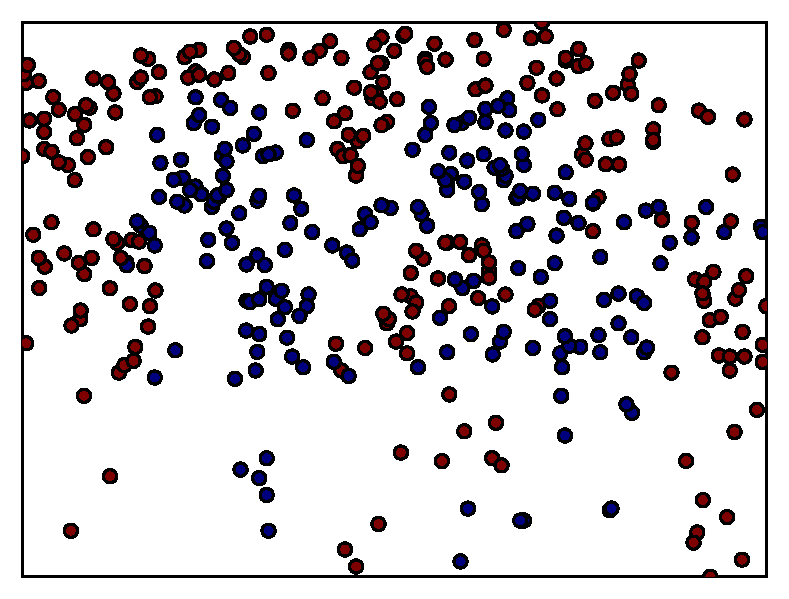
\includegraphics[width=0.45\textwidth]{img/boosting/1_data.pdf}&
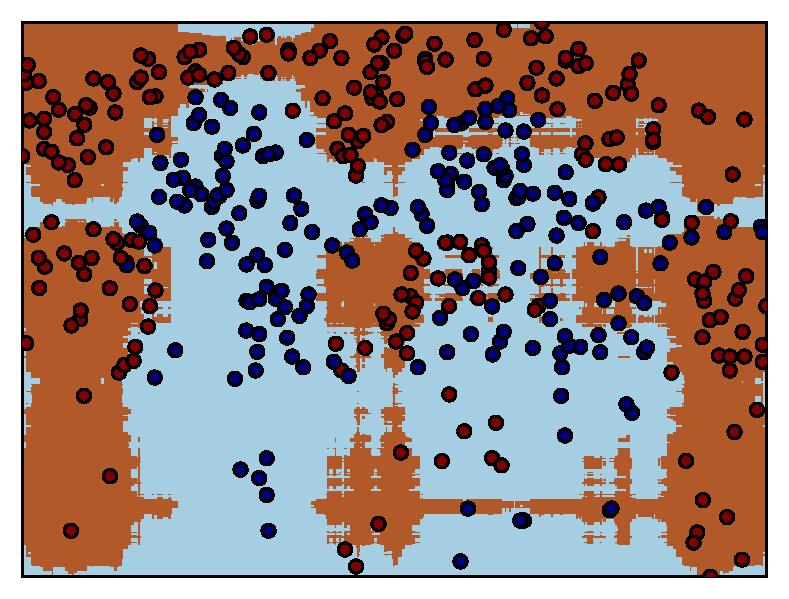
\includegraphics[width=0.45\textwidth]{img/boosting/1_boundary.pdf}
\end{tabular}
\end{figure}
\end{frame}

\begin{frame}{Adaboost: example (2)}
\begin{figure}
\begin{tabular}{cc}
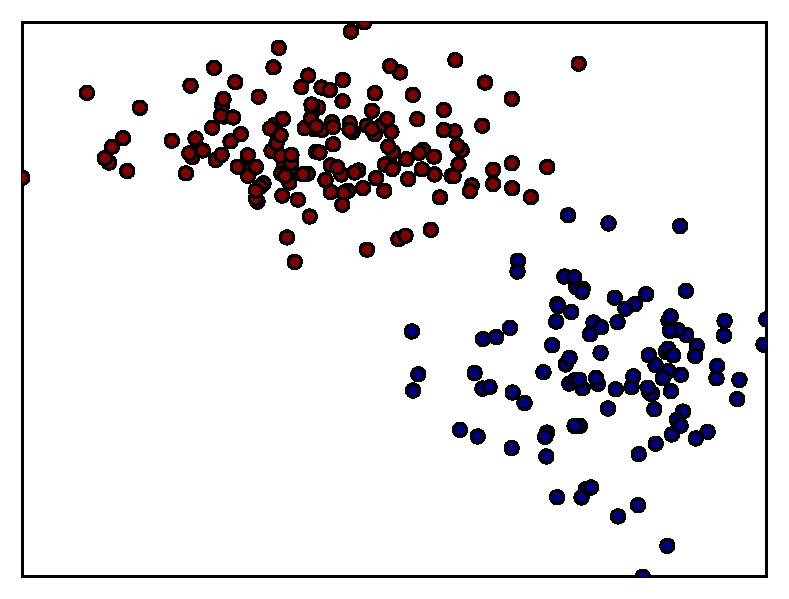
\includegraphics[width=0.45\textwidth]{img/boosting/2_data.pdf}&
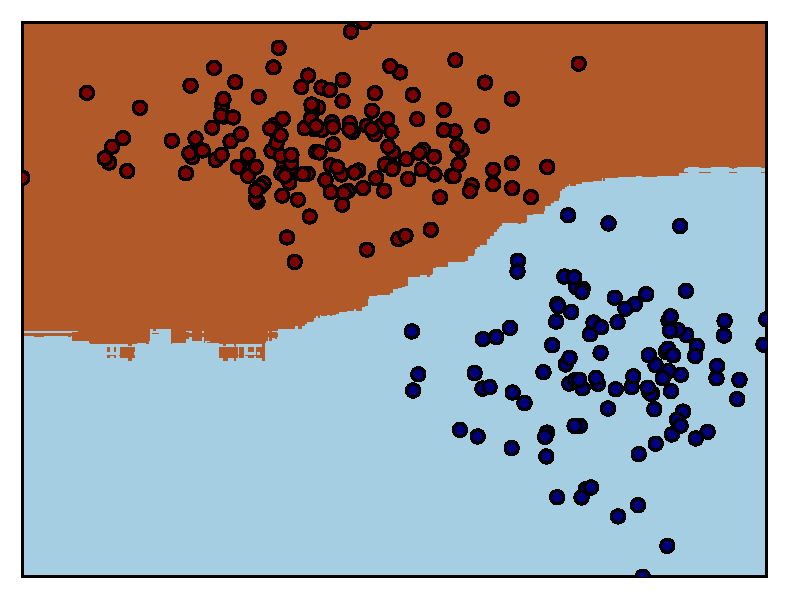
\includegraphics[width=0.45\textwidth]{img/boosting/2_boundary.pdf}
\end{tabular}
\end{figure}
\end{frame}

\begin{frame}{Adaboost: example (3)}
\begin{figure}
\begin{tabular}{cc}
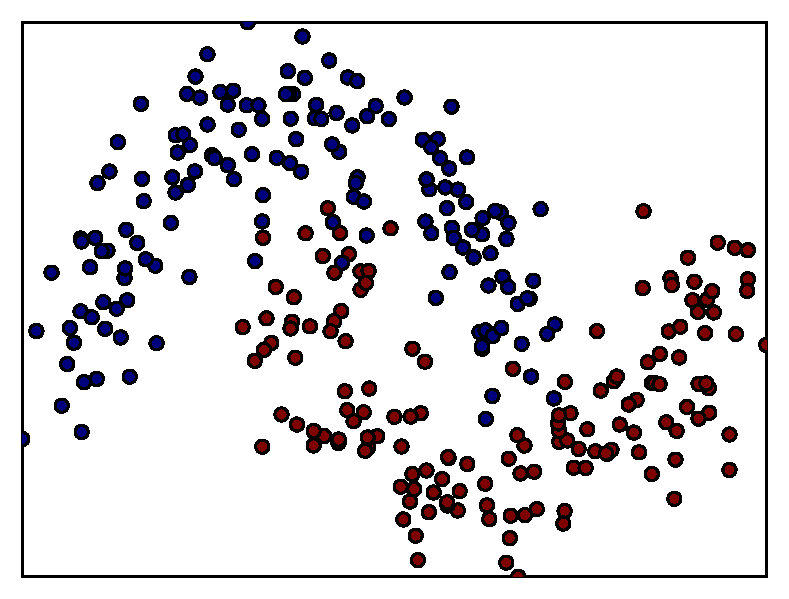
\includegraphics[width=0.45\textwidth]{img/boosting/3_data.pdf}&
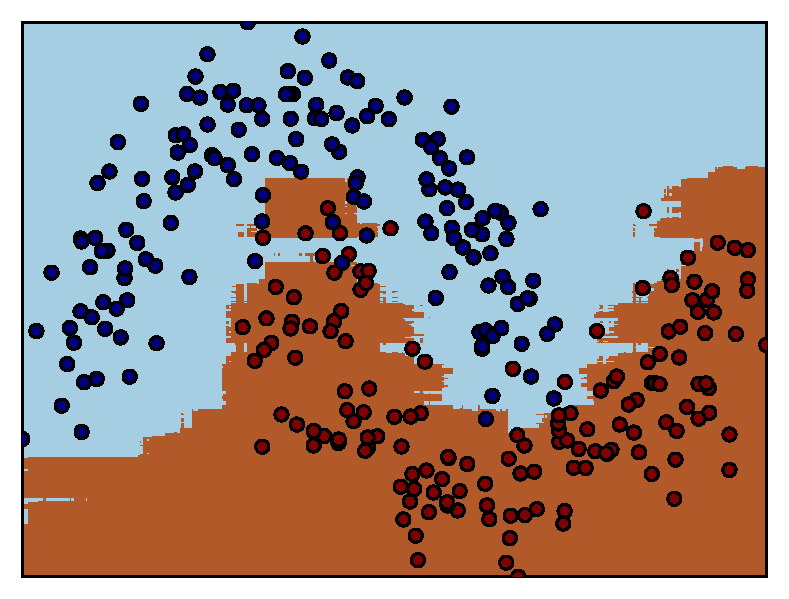
\includegraphics[width=0.45\textwidth]{img/boosting/3_boundary.pdf}
\end{tabular}
\end{figure}
\end{frame}


\end{document}